\documentclass[10pt,letterpaper]{article}

\usepackage[margin=0.75in]{geometry}
\usepackage{tikz}
\usepackage{graphicx}
\usepackage{amsmath}
\graphicspath{{images/}}
\begin{document}

  \title{Stats 314, Data Analysis \#1}
  \author{Cody Malick\\
  \texttt{malickc@oregonstate.edu}}
  \date{\today}
  \maketitle

\section*{Part I}
\subsection*{a}
Uniform distribution, because it is continuous, each time has an equal
probability, and distribution. This is a property unique to uniform
distributions.

\subsection*{b}
Poisson distribution, because we are given an average rate over a discrete
random variable. 

\subsection*{c}
Exponentional distribution, we're given a continuous random variable with an
average rate $(8)$, while also being given a skew indicating an exponential
distribution.

\subsection*{d}
Binomial distribution, as we are given a set of independent events, two 
possible outcomes, a probability of failure $(.25)$ and through that success
$(.75)$. 

\subsection*{e}
Normal distribution, as we are given an average value $(6)$, the standard
deviation from that value $(.6)$, and are told that values farther from the
median value are less likely. This describes a typical bell curve. 

\section*{Part II}
\subsection*{a}
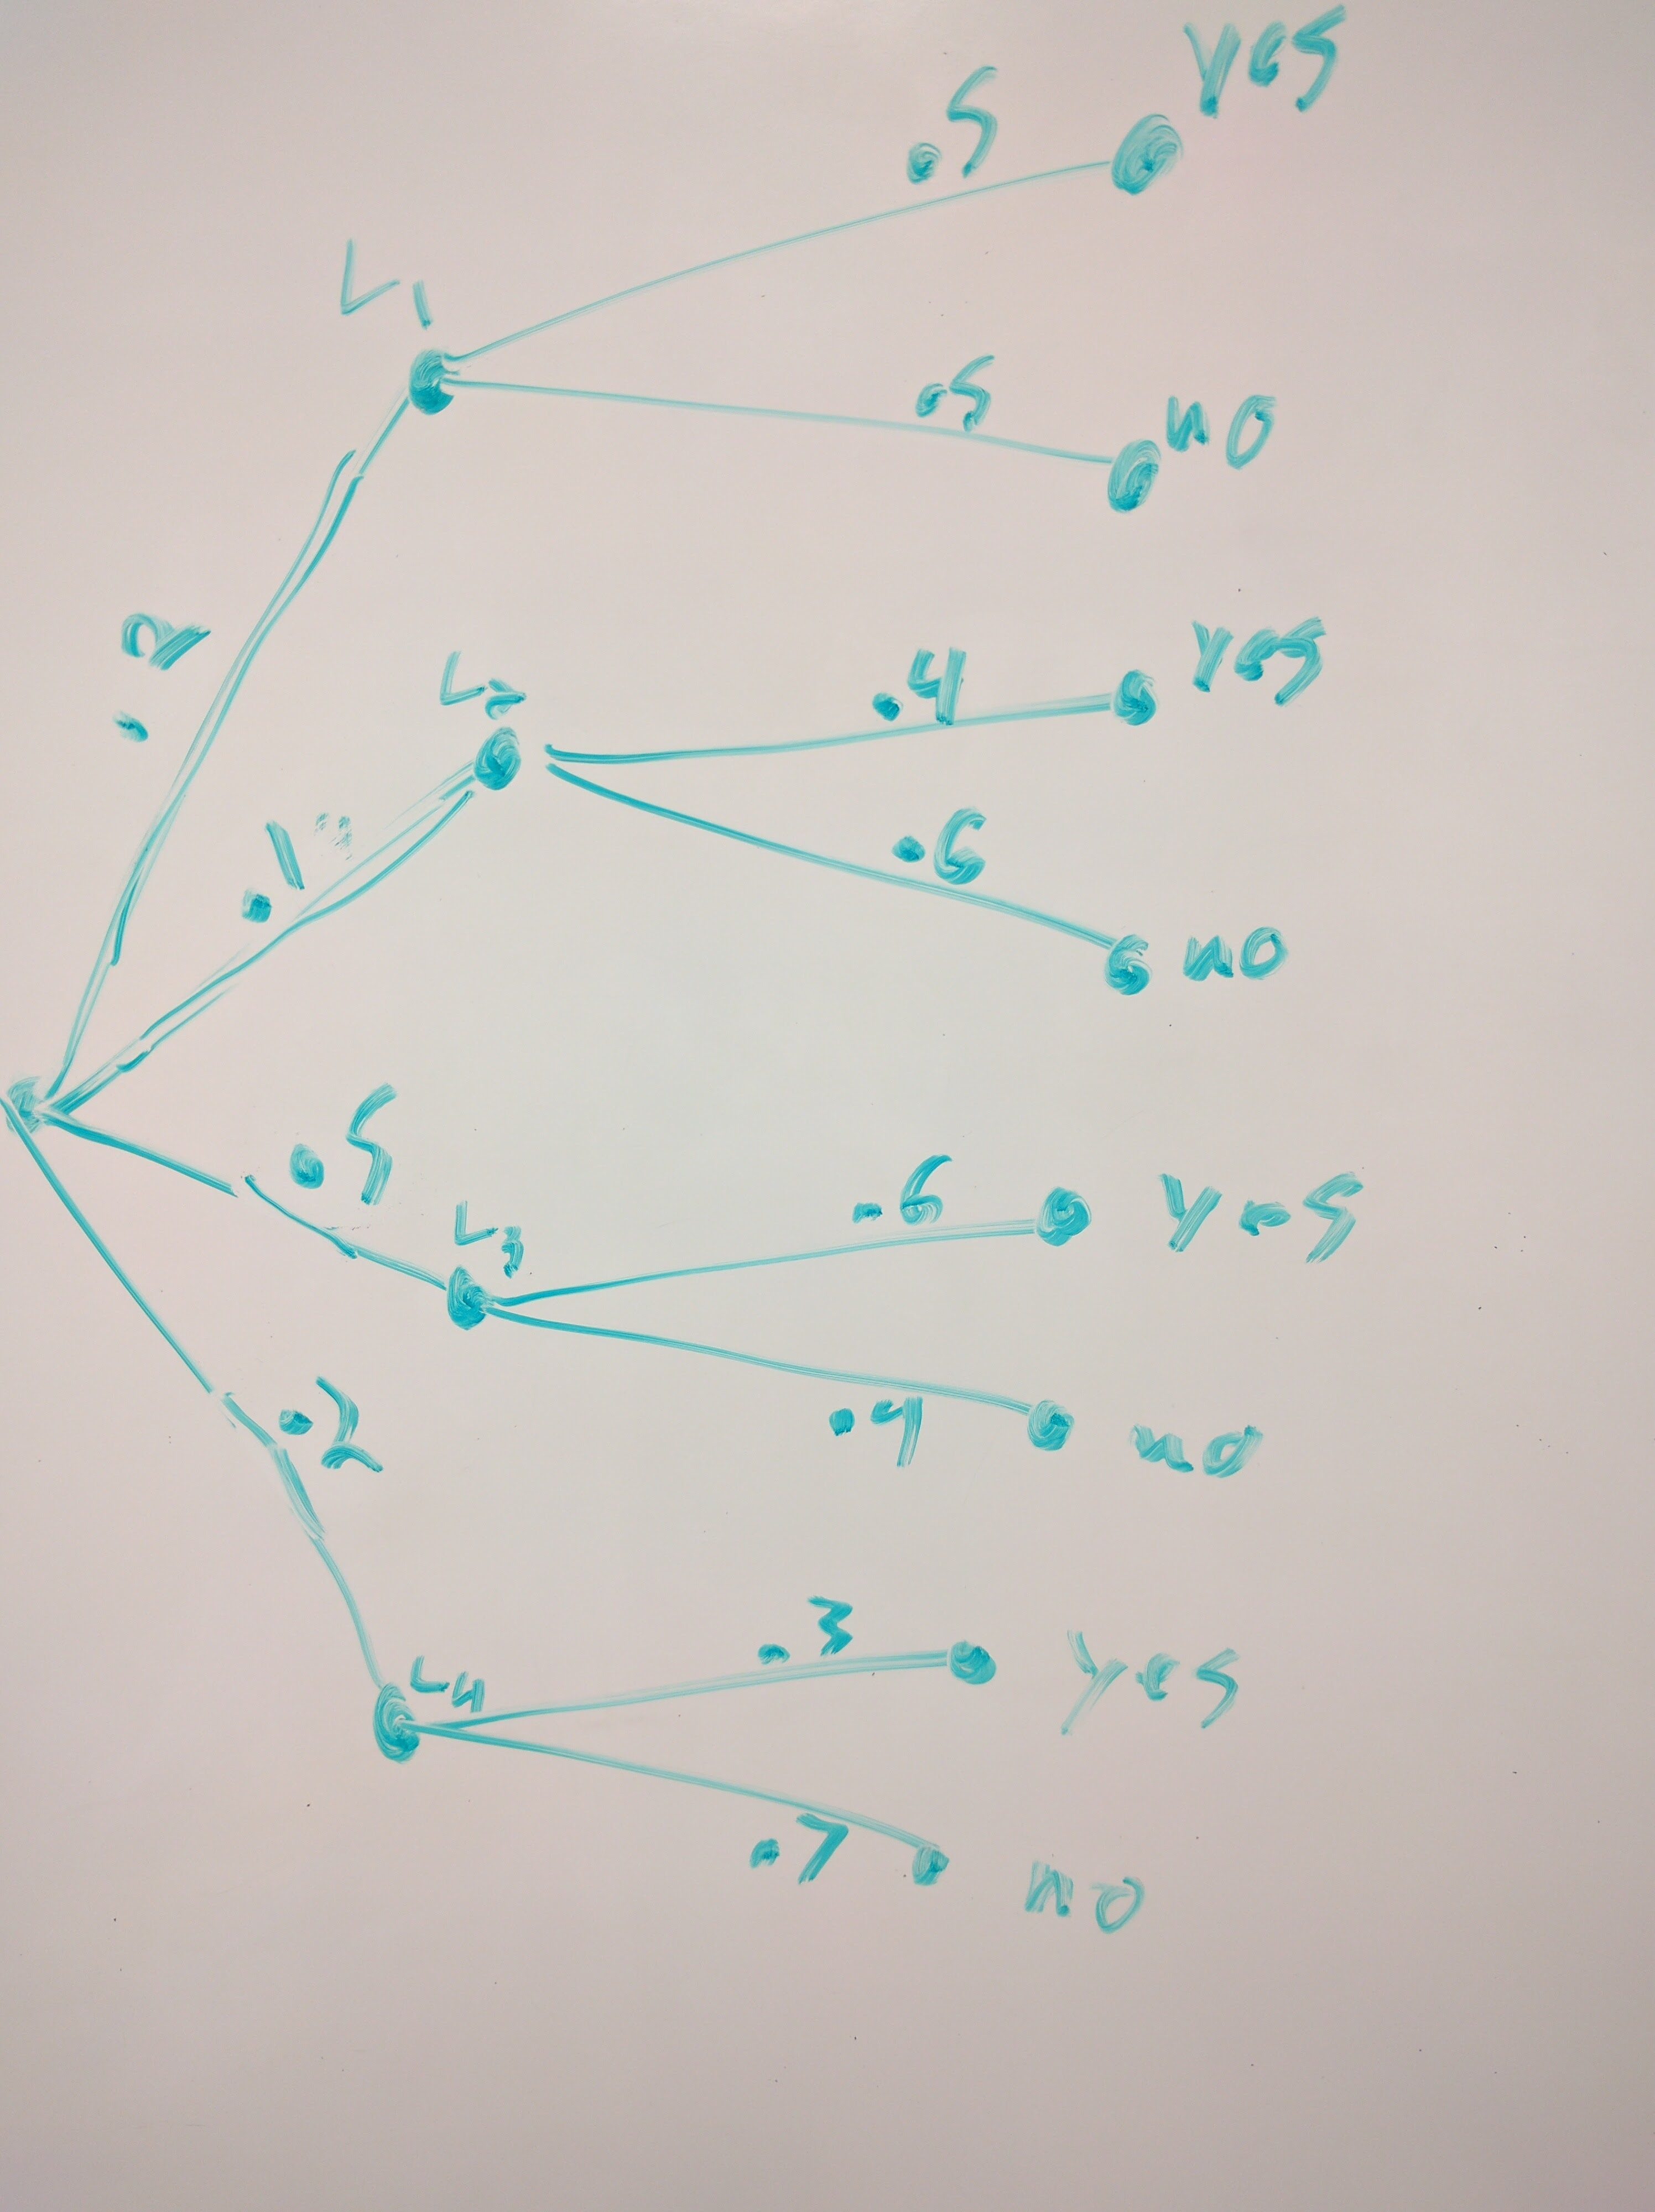
\includegraphics[scale=.075]{tree}

\subsection*{b}
To get the probability of a ticket, we have to use the law of total probability
to calculate the combined probability of getting a ticket in each area given
that they are in operation.

\noindent L1: $ .2*.5=.1 $\\
L2: $ .1*.4=.04 $\\
L3: $ .5*.6=.3 $\\
L4: $ .2*.3=.06 $\\
\\
P(ticket)=$ .1+.04+.3+.06=.5$

\section*{Part III}
\subsection*{a}
HHHH\\
HHHT\\
HHTH\\
HTHH\\
THHH\\
HHTT\\
HTHT\\
THHT\\
THTH\\
HTTH\\
TTHH\\
HTTT\\
THTT\\
TTHT\\
TTTH\\
TTTT\\
\subsection*{b}
$4/16=.25$
\subsection*{c}
$5/16=.3125$
\subsection*{d}
Binomial distribution, because we have a set of independent events with a discrete
random variable, and we're interested in the success rate for specific outcomes.
\subsection*{e}
To get the probability of $X = 3$, we have to take:\\
$P(X=3) = 4/16 = .25$
\subsection*{f}
To get the probability of $X >= 3$, we have to take:\\
$1-P(X>=3) = 1-(P(0)+P(1)+P(2)) = 1-.6875 = .3125$
\subsection*{g}
They sure are!
\subsection*{h}
The most likely number is 2. The likelihood is .375\\
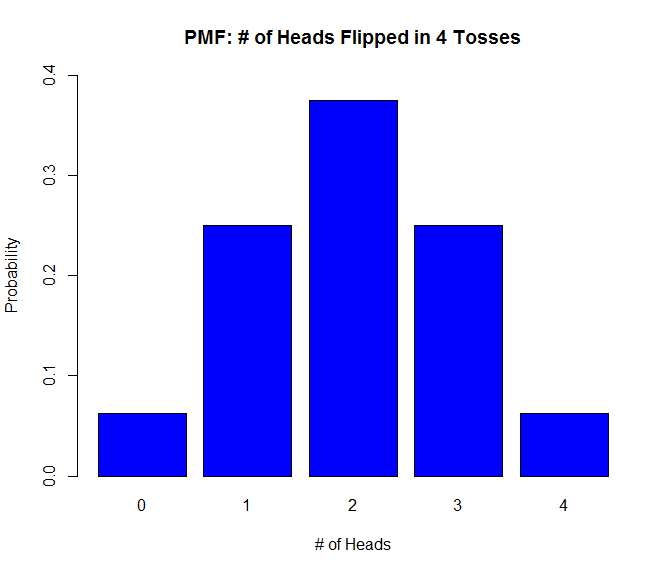
\includegraphics[scale=.75]{CoinPMF}

\subsection*{i}
$E(X)=np$, where $n$ is the number of coin tosses, and $p$ is the probability
of success.\\
$E(X)=4*.5=2$, which is our most likely number of heads/tails.

\section*{Part IV}
\subsection*{a}
To verify the distribution $f(x)$, we can simply integrate the two equations
from negative infinity to infinity get the range of the values we're interested
in.\\

For anything other than $0 < x < 1$, we can simply plug in zero, so that
simplifies the problem. We can take the integral of $5(1-x)^4$, from zero
to one because we know everything less than zero and greater than one equal
zero.\\

$\int_{-\infty}^{\infty}5(1-x)^4dx\\\\
=\int_{0}^{1}5(1-x)^4dx\\$\\
\\
Using u-substitution:\\
$5\int_{0}^{1}u^4du, u=(x-1), du=dx\\\\
=\dfrac{5(x-1)^5}{5}=(x-1)^5\big|_0^1\\\\
=(1-1)^5-(0-1)^5=0-(-1^5)=1$\\\\
This answer justifies our probability mass function because the total
probability equals 1. 

\subsection*{b}
The shape of the distribution is an inverse exponential curve. It is not,
however, an exponential distribution. There are no $e$ values in the equation.
Starting at five, decreasing towards zero.\\
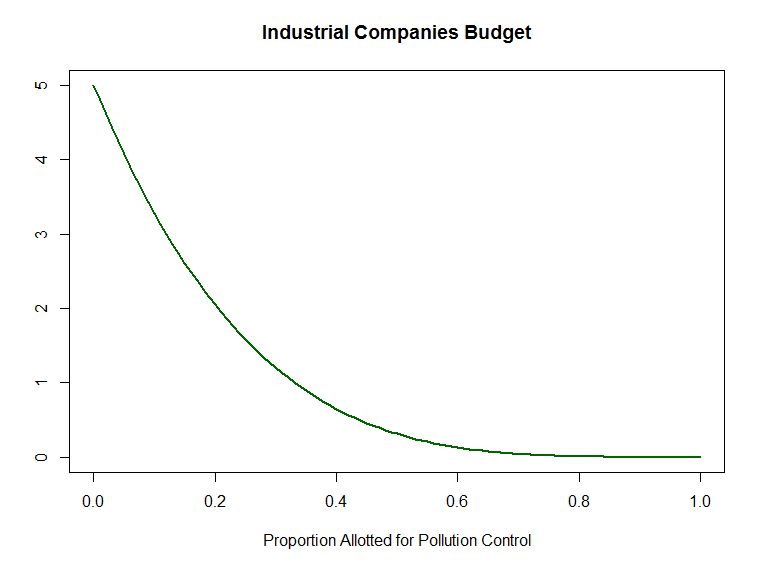
\includegraphics[scale=.75]{busPMF}
\subsection*{c}
The expected value of this distribution is $E(X)=\int_{-\infty}^{\infty}x*f(x)dx$.
Again, we can simply take the integral from 0 to 1 because of the bounds of our
integration.\\

$E(X)=\int_{-\infty}^{\infty}x*5(x-1)^4dx\\\\
=\int_{0}^{1}x5(x-1)^4dx = 5\int_{0}^{1}x(x-1)^4dx\\\\
=5\int_{0}^{1}(x-1)^4*(x-1+1) = 5\int_{0}^{1}(x-1)^5 + 5\int_{0}^{1}(x-1)^4\\\\$
Using u-substitution, where $u=x-1$:\\
$=5\int_{0}^{1}u^5du + =5\int_{0}^{1}u^4du=\dfrac{5(x-1)^6}{6}+(x-1)^5\big|_0^1\\\\
=(\dfrac{5(1-1)^6}{6}+(1-1)^5) - (\dfrac{5(0-1)^6}{6}+(0-1)^5 = 0 - (\dfrac{5}{6} - 1)\\\\
=-(-\dfrac{1}{6})=\dfrac{1}{6}$\\\\
So the expected value of our function is $\dfrac{1}{6}$

\subsection*{d}
The standard deviation of the function is: $SD=\sqrt{V(X)}$. So we need to find
$V(X)$.\\
$V(X)=E(X^2)-E(X) = E(X^2)-\dfrac{1}{6}\\\\
E(X^2) =\int_{0}^{1}(x^2)5(x-1)^4dx = 5\int_{0}^{1}(x^2)(x-1)^4dx\\\\$

Using u-substitution, where $u=x-1$:\\
$=5\int_{0}^{1}u^4 (u+1)^2 = 5\int_{0}^{1}u^6+2u^5+u^4du\\\\
=5\int_{0}^{1}u^6du+5\int_{0}^{1}2u^5du+5\int_{0}^{1}u^4du\\\\
=5(\dfrac{(x-1)^7}{7}+\dfrac{2(x-1)^6}{6}+\dfrac{(x-1)^5}{5})\big|_0^1\\\\
=\dfrac{5(x-1)^7}{7}+\dfrac{10(x-1)^6}{6}+(x-1)^5\big|_0^1\\\\
=(\dfrac{5(1-1)^7}{7}+\dfrac{10(1-1)^6}{6}+(1-1)^5)-(\dfrac{5(0-1)^7}{7}+\dfrac{10(0-1)^6}{6}+(0-1)^5)\\\\
=(0)-(\dfrac{-5}{7}+\dfrac{10}{6}-1=-(-.71428 + 1.6666 - 1) = .0476$\\\\

With our $E(X^2)$ we can calculate the variance and the standard deviation:\\

\noindent$V(X) = .0476-.02778 = .0198\\\\
SD(X) = \sqrt(.0198) = .1408$

\subsection*{e}
The CDF is the integral of the PDF from 0 to x, which we can quickly calculate
given previous work:\\\\
$\int_{0}^{x}f(x)dx = 5\int_{0}^{x}(1-x)^4 = (x-1)^5\big|_0^x = (x-1)^5 - (0-1)^5 = (x-1)^5+1$

Our CDF then is: $F(x)=(x-1)^5+1$

\subsection*{f}
We can find this quickly by plugging in $.05$ into our equation:\\
$(.05-1)^5+1=.2262$

\section*{Part V}
\subsection*{a}
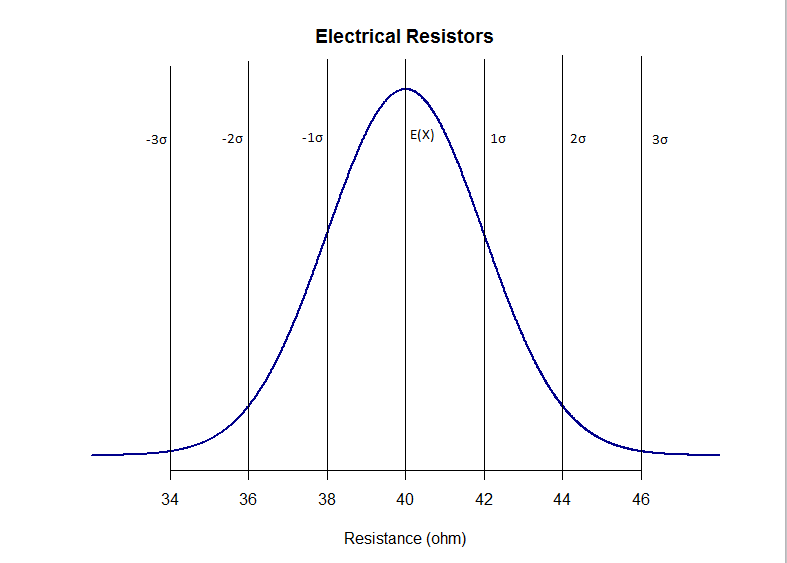
\includegraphics[scale=.75]{elecDIST}
\subsection*{b}
99.7\%
\subsection*{c}
At 43, we are 1.5 standard deviations from the median. With that info, we can
jump straight to the z-table. With a z-score of -1.5, or 1-zscore(1.5), then the
answer is $.06681$
\subsection*{d}
To find the percentile, we have to find what zscore occurs at about .25, which
in this case means $-.67*\sigma+\mu=-.67*2+40=38.66$



\end{document}
